\chapter{Kết quả}
\label{ch:results}

Mọi điểm đều lấy từ các tập kiểm định chính thức. Các dòng WEMoE cho giá trị trung bình và độ lệch chuẩn qua seed 0, 1 và 2.

\section{Kết quả theo tác vụ}

Bảng~\ref{tab:per-task} và Hình~\ref{fig:per-task} cho điểm theo tác vụ, và Bảng~\ref{tab:gain} đặt mỗi mô hình hợp nhất vào vị trí giữa lớp đa số và chuyên gia. Bản thân các chuyên gia không mạnh như nhau. SST-2 và QNLI, với nhiều dữ liệu huấn luyện nhất, đạt trên 90. RTE chỉ đạt 63.2, và điểm dev của nó vẫn đang tăng ở epoch cuối (49.0, 65.5, 65.9). Huấn luyện chuyên gia mất tổng cộng 43 phút: 0.8, 0.7, 1.1, 11.0 và 29.8 phút cho MRPC, RTE, CoLA, SST-2 và QNLI, với epoch tốt nhất lần lượt là 2, 3, 3, 2 và 3.

\begin{table}[htbp]
  \centering\tablestyle
  \caption{Điểm theo tác vụ ($\times100$). In đậm là các kết quả WEMoE $k=256$ thấp hơn lớp đa số.}
  \label{tab:per-task}
  \setlength{\tabcolsep}{3pt}\begin{tabular}{l c c c c c}
    \toprule
    Mô hình & MRPC (Acc/F1) & RTE (Acc) & CoLA (MCC) & SST-2 (Acc) & QNLI (Acc)\\
    \midrule
    Lớp đa số & 68.4 / 81.2 & 52.7 & 0.0 & 50.9 & 50.5\\
    Simple Averaging & 68.4 / 81.2 & 46.9 & 23.3 & 55.4 & 65.9\\
    Task Arithmetic & 68.6 / 81.3 & 47.3 & 16.9 & 69.8 & 77.9\\
    Input-independent, $k$=256 & 68.4 / 81.2 & 47.3 & 20.2$\pm$0.0 & 70.9$\pm$0.1 & 78.6$\pm$0.0\\
    WEMoE full, $k$=16 & 68.7$\pm$2.3 / 80.6$\pm$2.2 & 48.0$\pm$1.0 & 27.6$\pm$14.1 & 79.6$\pm$8.1 & 74.0$\pm$6.5\\
    WEMoE full, $k$=64 & 71.6$\pm$4.4 / 80.9$\pm$4.3 & 54.0$\pm$3.4 & 20.5$\pm$17.8 & 89.0$\pm$0.6 & 83.1$\pm$2.4\\
    WEMoE full, $k$=256 & 76.3$\pm$4.5 / 83.9$\pm$2.8 & \textbf{52.0$\pm$4.4} & 42.6$\pm$0.9 & 88.0$\pm$0.5 & 86.7$\pm$0.7\\
    WEMoE intermediate, $k$=256 & \textbf{66.5$\pm$0.7 / 76.6$\pm$1.0} & 59.0$\pm$0.9 & 41.7$\pm$0.9 & 86.7$\pm$0.2 & 86.5$\pm$0.2\\
    Các chuyên gia riêng & 82.1 / 88.1 & 63.2 & 59.1 & 92.2 & 91.2\\
    \bottomrule
  \end{tabular}
\end{table}

\begin{figure}[htbp]
  \centering
  \input{figures_vi/per_task}
  \caption{Điểm tác vụ của các mô hình hợp nhất giữa lớp đa số (vạch đứt) và các chuyên gia (vạch liền). Giá trị WEMoE dùng $k=256$ và là trung bình qua ba seed.}
  \label{fig:per-task}
\end{figure}

\begin{table}[htbp]
  \centering\tablestyle
  \caption{Mức tăng so với lớp đa số theo tác vụ, tính bằng phần trăm từ trung bình các seed.}
  \label{tab:gain}
  \begin{tabular}{l r r r r r r}
    \toprule
    Mô hình & MRPC & RTE & CoLA & SST-2 & QNLI & Trung bình\\
    \midrule
    Task Arithmetic & 1.8 & $-51.7$ & 28.6 & 45.8 & 67.3 & 18.4\\
    Input-independent, $k=256$ & 0.0 & $-51.7$ & 34.2 & 48.5 & 68.9 & 20.0\\
    WEMoE full, $k=256$ & 51.5 & $-6.9$ & 72.2 & 89.7 & 88.9 & 59.1\\
    WEMoE intermediate, $k=256$ & $-31.6$ & 59.8 & 70.5 & 86.8 & 88.5 & 54.8\\
    \bottomrule
  \end{tabular}
\end{table}

Cải thiện trung bình không áp dụng đồng đều. Trên SST-2 và QNLI, các bộ định tuyến đã huấn luyện khôi phục gần 90\% mức tăng, và trên CoLA khoảng 70\%, so với 45.8, 67.3 và 28.6 của Task Arithmetic. Hợp nhất tĩnh gần với dự đoán hằng trên hai tác vụ nhỏ nhất. Độ chính xác 47.3 của nó trên RTE bằng 131/277, đúng tỉ lệ của lớp \emph{thiểu số}, phù hợp với việc dự đoán một nhãn cho mọi mẫu, và điểm MRPC của nó gần như không khác lớp đa số. WEMoE không khắc phục hoàn toàn điều này. Mô hình full MLP khôi phục khoảng một nửa mức tăng trên MRPC nhưng không vượt lớp đa số một cách ổn định trên RTE: ba seed cho 49.5, 57.0 và 49.5, so với 52.7. Mô hình intermediate-only khôi phục 59.8\% trên RTE nhưng thấp hơn lớp đa số trên MRPC. Không mô hình hợp nhất nào bằng chuyên gia ở bất kỳ tác vụ nào.

\section{So sánh với các baseline}

Bảng~\ref{tab:main} là so sánh tổng hợp. Task Arithmetic đạt 57.4 và chỉ khôi phục 18.4\% mức tăng, dù điểm chuẩn hóa 70.6 của nó gợi ý nhiều hơn thế. Trước khi huấn luyện, mô hình full MLP gần với nó ($57.8\pm0.6$) nhưng không trùng, vì các trọng số ngẫu nhiên nhỏ của bộ định tuyến làm thay đổi đặc biệt là điểm CoLA. Ở $k=256$, FSFT nâng mô hình lên $69.9\pm0.1$, cao hơn Task Arithmetic 12.5 điểm và thấp hơn các chuyên gia 8.3 điểm, với mức tăng $59.1\pm1.1$.

\begin{table}[htbp]
  \centering\tablestyle
  \caption{Kết quả tổng hợp ($\times100$). ``Init'' là WEMoE trước khi huấn luyện bộ định tuyến. Thời gian là một lần chạy FSFT trên T4, gồm cả các lần đánh giá dev.}
  \label{tab:main}
  \begin{tabular}{l c c c c r}
    \toprule
    Mô hình & Trung bình & Chuẩn hóa & Gain & Bước tốt nhất / 500 & Phút\\
    \midrule
    Lớp đa số & 45.8 & 56.4 & 0.0 & -- & --\\
    Simple Averaging & 53.3 & 66.8 & 6.6 & -- & --\\
    Task Arithmetic ($\lambda=0.3$) & 57.4 & 70.6 & 18.4 & -- & --\\
    Init, full MLP & 57.8$\pm$0.6 & 71.3$\pm$1.0 & 18.7$\pm$1.5 & -- & --\\
    Init, intermediate-only & 57.5$\pm$0.4 & 70.8$\pm$0.6 & 18.1$\pm$1.2 & -- & --\\
    Input-independent, $k=256$ & 58.4$\pm$0.0 & 72.0$\pm$0.0 & 20.0$\pm$0.0 & 50, 50, 50 & 15.4\\
    WEMoE full, $k=16$ & 60.8$\pm$2.7 & 75.6$\pm$4.6 & 25.5$\pm$4.6 & 50, 0, 150 & 16.3\\
    WEMoE full, $k=64$ & 64.6$\pm$3.7 & 79.5$\pm$6.3 & 46.7$\pm$8.5 & 100, 250, 100 & 14.4\\
    \textbf{WEMoE full, $k=256$} & \textbf{69.9$\pm$0.1} & \textbf{87.8$\pm$0.5} & \textbf{59.1$\pm$1.1} & 250, 200, 200 & 16.3\\
    WEMoE intermediate, $k=256$ & 69.1$\pm$0.1 & 87.4$\pm$0.1 & 54.8$\pm$1.7 & 500, 400, 400 & 8.4\\
    Các chuyên gia riêng & 78.2 & 100.0 & 100.0 & -- & --\\
    \bottomrule
  \end{tabular}
\end{table}

\paragraph{Ablation không phụ thuộc đầu vào.} Các hệ số cố định cho mọi đầu vào gần như không làm điểm thay đổi ($58.4\pm0.0$, mức tăng 20.0). Chúng bắt đầu từ điểm dev của Task Arithmetic (62.8), nằm trong khoảng 62.4 đến 63.0 suốt quá trình huấn luyện, và đạt điểm tốt nhất ở bước 50 trên mọi seed. Các hệ số học được chỉ lệch tối đa 0.023 so với giá trị ban đầu 0.3. Trong cùng 500 bước, các bộ định tuyến full MLP bắt đầu từ 62.6 đến 62.9 trên dev và đạt điểm tốt nhất 72.6, 73.0 và 72.9. Biến thể này chỉ được thử với một learning rate.

\paragraph{Ngân sách few-shot.} Hình~\ref{fig:k-sweep} cho thấy điểm trung bình tăng theo $k$ và chưa chững lại ở 256. Ngân sách nhỏ dao động mạnh giữa các seed. Ảnh hưởng của ngân sách cũng không đơn điệu ở mọi tác vụ: MCC của CoLA có trung bình 27.6 ở $k=16$ và 20.5 ở $k=64$, với các lần chạy trải từ 18--44 và 9--41, rồi đạt $42.6\pm0.9$ ở $k=256$. Với seed 1 ở $k=16$, không bước nào vượt bộ định tuyến chưa huấn luyện trên dev, nên lần chạy đó báo cáo WEMoE init. Ở $k=256$, mọi tác vụ có độ lệch chuẩn tối đa 0.9, trừ MRPC và RTE, nên điểm trung bình ổn định che khuất sự dao động trên hai tác vụ này.

\begin{figure}[htbp]
  \centering
  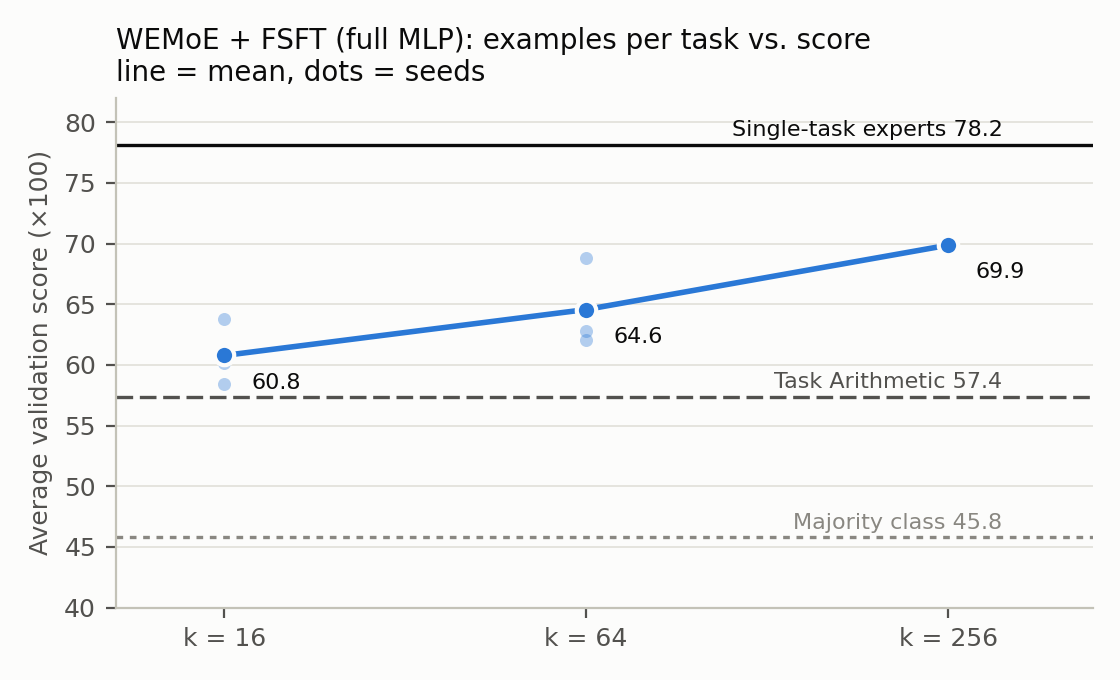
\includegraphics[width=.4\linewidth]{k_sweep.png}
  \caption{Điểm trung bình trên tập kiểm định của WEMoE full MLP theo ngân sách few-shot. Đường là giá trị trung bình, các chấm là từng seed.}
  \label{fig:k-sweep}
\end{figure}

\section{Hành vi định tuyến}
\label{sec:routing}

Hình~\ref{fig:routing} cho thấy giá trị trung bình của bộ định tuyến theo lớp và tác vụ đầu vào của một mô hình đã huấn luyện. Nhiều giá trị nằm xa giá trị ban đầu khoảng $\lambda$, và có cả hai dấu, điều mà một tổ hợp lồi không thể biểu diễn. Các ô trông khá giống nhau, nên phần lớn mẫu hình được chia sẻ giữa các tác vụ đầu vào, dù chúng cũng khác nhau ở một số chỗ, cho thấy định tuyến phụ thuộc một phần vào đầu vào. Trong mô hình này, cột của chuyên gia RTE mang giá trị âm ở hai lớp cuối với mọi loại đầu vào.

\begin{figure}[htbp]
  \centering
  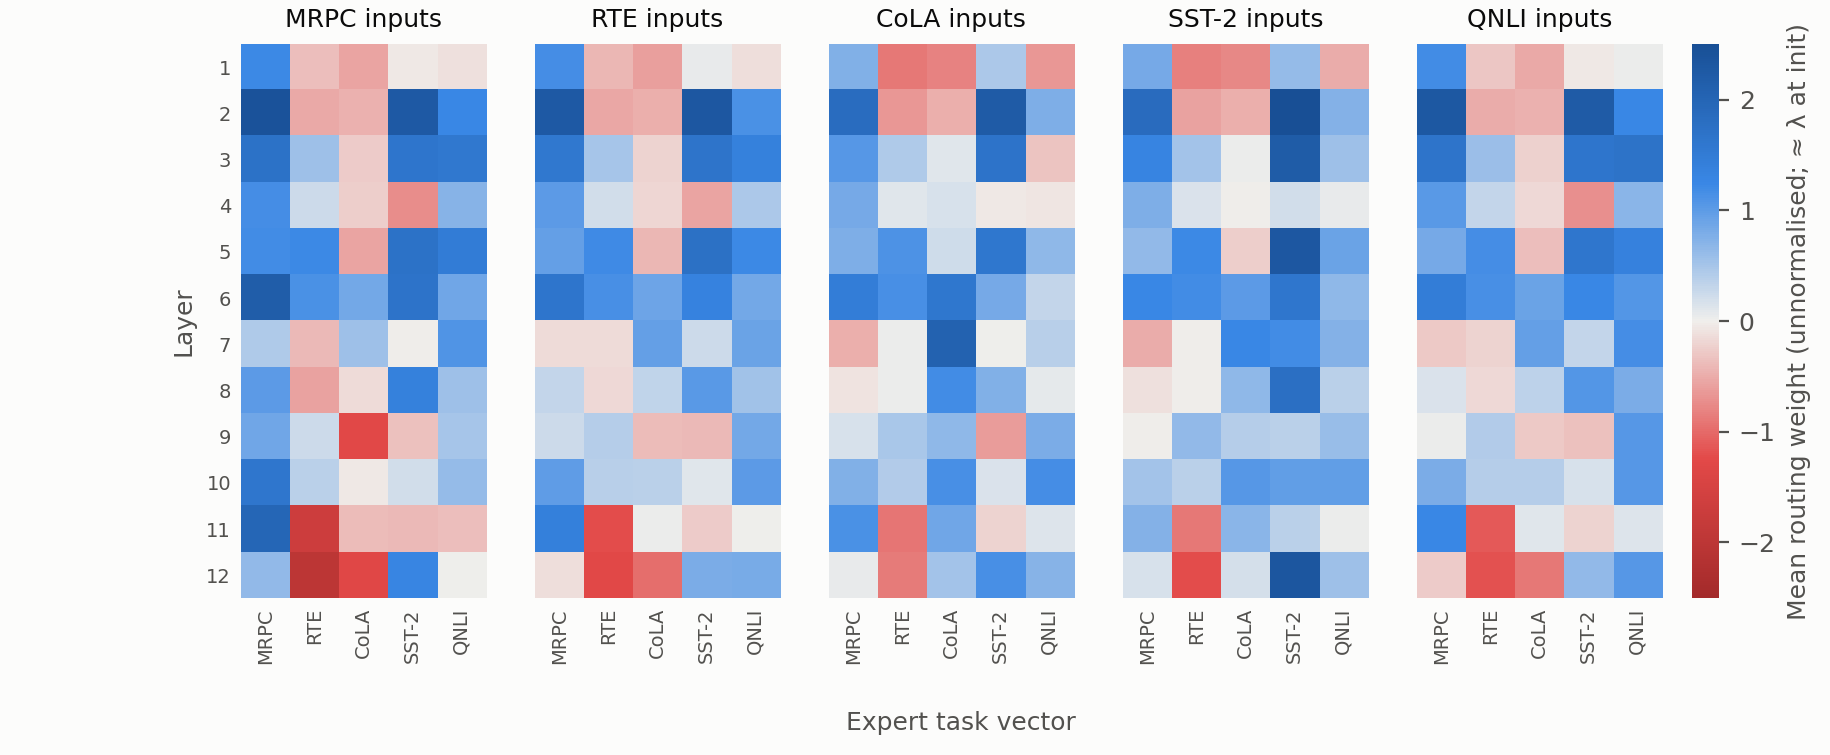
\includegraphics[width=.6\linewidth]{routing_clean.png}
  \caption{Giá trị trung bình của bộ định tuyến theo lớp và tác vụ đầu vào (full MLP, $k=256$, seed 0). Màu xanh cộng và màu đỏ trừ một véc-tơ tác vụ.}
  \label{fig:routing}
\end{figure}

Chúng tôi định lượng mẫu hình này từ giá trị bộ định tuyến của từng mẫu kiểm định. Với seed 0, các giá trị riêng lẻ trải từ $-3.0$ đến $4.4$, và tổng theo lớp của các giá trị trung bình trên toàn bộ mẫu đạt 5.8, so với 1.5 lúc khởi tạo. Ma trận định tuyến trung bình của các tác vụ đầu vào khác nhau có tương quan trung bình 0.82 (0.84 với seed 1 và 2), trong khi tác vụ đầu vào giải thích khoảng 58\% phương sai định tuyến (60\% với seed 1 và 2). Bảng~\ref{tab:own} cho thấy phần lớn các tác vụ tăng trọng số cho chuyên gia của chính mình, trừ RTE.

Chuyên gia RTE hành xử khác nhau giữa hai phạm vi, và một seed là chưa đủ để đọc khác biệt này. Giá trị của nó trên đầu vào RTE ở lớp 12 mang dấu âm với full MLP ở cả ba seed ($-1.28$, $-0.65$, $-0.76$) và dấu dương với intermediate-only ($2.04$, $1.16$, $1.53$). Giá trị trung bình theo lớp kém ổn định hơn: với intermediate-only, nó là 0.96, 0.27 và 0.31, trong khi độ chính xác RTE nằm trong khoảng 58.1 đến 59.9, nên trung bình này không giải thích được kết quả RTE. Bằng chứng này chỉ cho thấy mối liên hệ và không xác lập vì sao RTE thất bại.

\begin{table}[htbp]
  \centering\tablestyle
  \caption{Giá trị trung bình của bộ định tuyến dành cho chuyên gia của chính tác vụ, lấy trung bình qua các lớp (full MLP, $k=256$, seed 0).}
  \label{tab:own}
  \begin{tabular}{l c c c c c}
    \toprule
    & MRPC & SST-2 & QNLI & CoLA & RTE\\
    \midrule
    Trên đầu vào của chính nó & 1.37 & 1.37 & 0.94 & 0.61 & 0.01\\
    Trên đầu vào của tác vụ khác & 0.77 & 0.67 & 0.56 & $-0.02$ & $-0.01$\\
    \bottomrule
  \end{tabular}
\end{table}

\section{Lưu trữ, số tham số và độ trễ suy luận}
\label{sec:efficiency}

Bảng~\ref{tab:storage} phân tách các tham số được lưu, khớp với Phương trình~\eqref{eq:storage} và được đo trên các mô hình đã dựng. Véc-tơ tác vụ chiếm ưu thế, với 283.3M trong 400.0M tham số của mô hình full MLP.

\begin{table}[htbp]
  \centering\tablestyle
  \caption{Số tham số lưu trữ (triệu) theo thành phần, và tổng dung lượng ở độ chính xác 32-bit.}
  \label{tab:storage}
  \setlength{\tabcolsep}{4pt}\begin{tabular}{l r r r r r r r r}
    \toprule
    Triển khai & Tĩnh & MLP gốc & Véc-tơ tác vụ & Định tuyến & Head & Tổng & GiB & So với 5 MH\\
    \midrule
    5 mô hình riêng & -- & -- & -- & -- & -- & 547.4 & 2.04 & 100.0\%\\
    Task Arithmetic & -- & -- & -- & -- & -- & 109.5 & 0.41 & 20.0\%\\
    WEMoE, full MLP & 52.8 & 56.7 & 283.3 & 7.13 & 0.008 & 400.0 & 1.49 & 73.1\%\\
    WEMoE, intermediate-only & 81.1 & 28.3 & 141.7 & 7.13 & 0.008 & 258.4 & 0.96 & 47.2\%\\
    \bottomrule
  \end{tabular}
\end{table}

Bảng~\ref{tab:latency} báo cáo độ trễ trên một GPU T4, với các token id ngẫu nhiên dài 128, mixed precision và head MRPC, là trung bình của 10 lượt truyền xuôi sau 3 lượt khởi động. Dòng mô hình riêng đo một chuyên gia, vì mỗi đầu vào sẽ đi đến đúng chuyên gia của nó theo mã tác vụ. Số liệu batch 1 chỉ mang tính tham khảo: chúng lệch tới 27\% giữa hai lần đo (24.05 ms và 18.90 ms với mô hình intermediate-only), trong khi số liệu batch 32 khớp trong khoảng 5\%. Ở batch 32, mô hình full MLP chậm hơn một BERT khoảng 4.5 lần và mô hình intermediate-only khoảng 2.9 lần, và mô hình full MLP cần khoảng 2.8 lần bộ nhớ GPU cao nhất.

\begin{table}[htbp]
  \centering\tablestyle
  \caption{Độ trễ suy luận và bộ nhớ GPU cao nhất trên một T4, từ lần đo cuối. $^{*}$Đo một chuyên gia.}
  \label{tab:latency}
  \begin{tabular}{l c c c c}
    \toprule
    & \multicolumn{2}{c}{Batch 1} & \multicolumn{2}{c}{Batch 32}\\
    Triển khai & ms/mẫu & MB cao nhất & ms/mẫu & MB cao nhất\\
    \midrule
    BERT riêng theo tác vụ$^{*}$ & 11.64 & 614 & 1.61 & 704\\
    Task Arithmetic & 12.67 & 435 & 1.63 & 519\\
    WEMoE, full MLP & 27.83 & 1615 & 7.31 & 1987\\
    WEMoE, intermediate-only & 18.90 & 1061 & 4.69 & 1387\\
    \bottomrule
  \end{tabular}
\end{table}
